\documentclass{article}

\usepackage[spanish]{babel}
\usepackage[utf8]{inputenc}
\usepackage[right=1.5cm,left=1.5cm,top=1.5cm,bottom=1.5cm]{geometry}

\title{Tercer Taller\\ Estadística genómica}
\author{Juan David Henao Sánchez}

\usepackage{Sweave}
\begin{document}
\Sconcordance{concordance:JuanHenao_Taller3.tex:JuanHenao_Taller3.Rnw:%
1 9 1 1 0 9 1 1 2 1 0 1 1 3 0 2 2 1 0 2 1 7 0 1 1 19 0 1 1 7 0 2 2 4 0 %
2 2 1 0 1 1 4 0 2 2 1 0 1 1 4 0 1 2 5 1 1 2 1 0 4 1 5 0 1 1 6 0 2 2 1 0 %
2 1 4 0 1 2 5 1 1 2 4 0 2 2 1 0 1 1 6 0 2 2 4 0 2 2 1 0 2 1 1 2 4 0 1 2 %
1 1}


\maketitle

\section*{Sobre datos del GEO del NCBI de su elección (que comparen dos condiciones biológicas con al menos 5 réplicas) realice los siguientes pasos luego de normalizar:}
\subsection*{1. Realice un MA-plot}


\begin{Schunk}
\begin{Sinput}
> library(GEOquery)
> library(vsn)
> ########################
> gds <- getGEO("GDS3750")
> eset <- GDS2eSet(gds, do.log2 = TRUE)
> eset
\end{Sinput}
\begin{Soutput}
ExpressionSet (storageMode: lockedEnvironment)
assayData: 22277 features, 8 samples 
  element names: exprs 
protocolData: none
phenoData
  sampleNames: GSM430339 GSM430340 ... GSM430346 (8 total)
  varLabels: sample genotype/variation description
  varMetadata: labelDescription
featureData
  featureNames: 1007_s_at 1053_at ... AFFX-TrpnX-M_at (22277 total)
  fvarLabels: ID Gene title ... GO:Component ID (21 total)
  fvarMetadata: Column labelDescription
experimentData: use 'experimentData(object)'
  pubMedIds: 20395301 
Annotation:  
\end{Soutput}
\begin{Sinput}
> dim(eset)
\end{Sinput}
\begin{Soutput}
Features  Samples 
   22277        8 
\end{Soutput}
\begin{Sinput}
> ##########################
> nml <- justvsn(eset)
\end{Sinput}
\end{Schunk}

\begin{Schunk}
\begin{Sinput}
> meanSdPlot(eset)
> title(main='Datos normalizados',font=2)
\end{Sinput}
\end{Schunk}
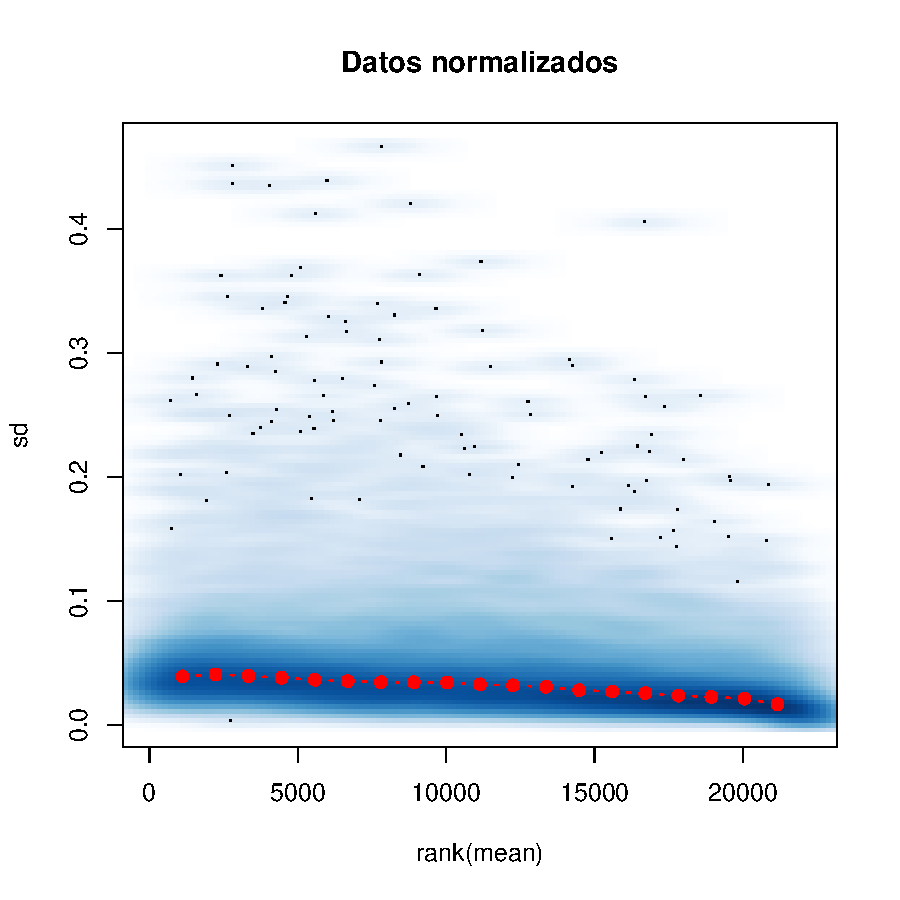
\includegraphics{JuanHenao_Taller3-002}

\textbf{MA PLOT}

\begin{Schunk}
\begin{Sinput}
> ###############################
> iref = seq(1, 7, by=2)
> ismp = seq(2, 8, by=2)
> M= exprs(nml)[,ismp]-exprs(nml)[,iref] 
> A=(exprs(nml)[,ismp]+exprs(nml)[,iref])/2
> dim(M)
\end{Sinput}
\begin{Soutput}
[1] 22277     4
\end{Soutput}
\begin{Sinput}
> dim(A)
\end{Sinput}
\begin{Soutput}
[1] 22277     4
\end{Soutput}
\end{Schunk}

\begin{Schunk}
\begin{Sinput}
> smoothScatter(rowMeans(A), rowMeans(M), main=" ", xlab="A", ylab="M", pch=20)
> title(main='MA PLOT',font=2)
> abline(h=0, col="red")
\end{Sinput}
\end{Schunk}
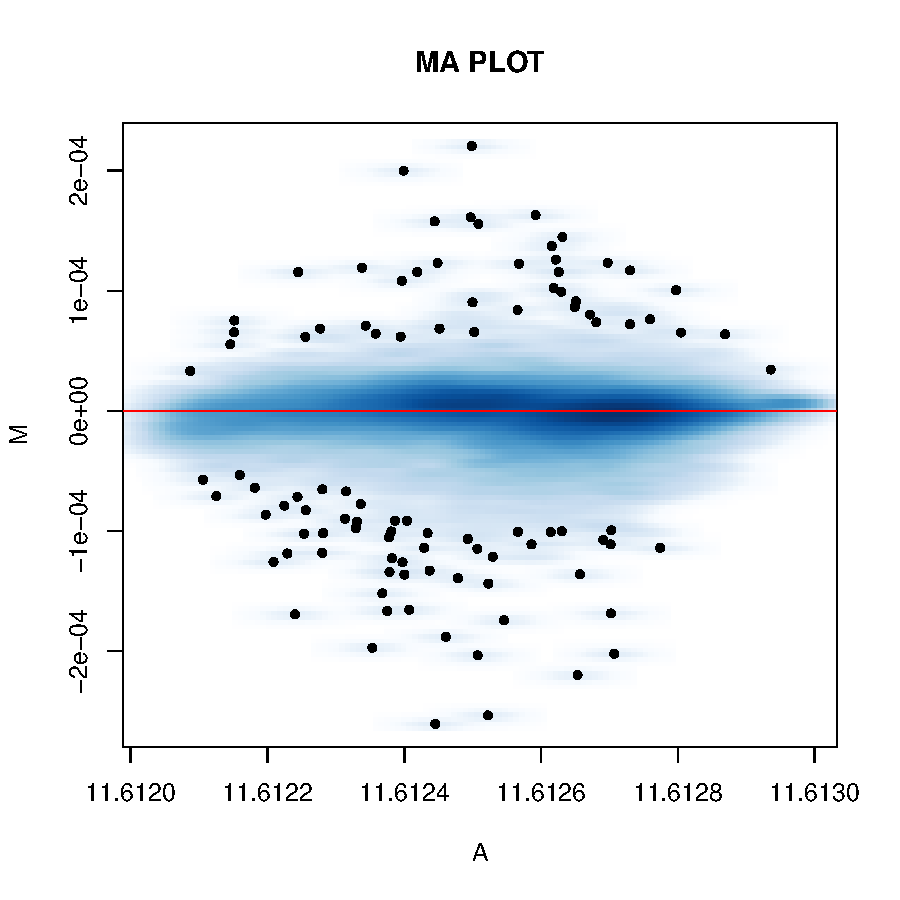
\includegraphics{JuanHenao_Taller3-004}

\subsection*{2. Identifique los genes diferencialmente expresados con pruebas T múltiples (rowttest) y resáltelos en el MAplot}

\begin{Schunk}
\begin{Sinput}
> library(genefilter)
> library("GSEABase")
> library(ALL)
> data(ALL)
> ####################################
> bcell=grep("B", as.character(ALL$BT))
> moltyp=which(as.character(ALL$mol.biol) %in% c("NEG", "BCR/ABL"))
> ALL_bcrneg=ALL[,intersect(bcell,moltyp)]
> ALL_bcrneg$mol.biol=factor(ALL_bcrneg$mol.biol)
> class(ALL_bcrneg)
\end{Sinput}
\begin{Soutput}
[1] "ExpressionSet"
attr(,"package")
[1] "Biobase"
\end{Soutput}
\begin{Sinput}
> #####################################
> gsc=GeneSetCollection(ALL_bcrneg, setType=KEGGCollection())
> gsc
\end{Sinput}
\begin{Soutput}
GeneSetCollection
  names: 04610, 00232, ..., 00785 (228 total)
  unique identifiers: 189_s_at, 31825_at, ..., 41859_at (5333 total)
  types in collection:
    geneIdType: AnnotationIdentifier (1 total)
    collectionType: KEGGCollection (1 total)
\end{Soutput}
\begin{Sinput}
> Am= incidence(gsc)
> dim(Am)
\end{Sinput}
\begin{Soutput}
[1]  228 5333
\end{Soutput}
\begin{Sinput}
> ######################################
> nsF=ALL_bcrneg[colnames(Am),]
> dim(nsF)
\end{Sinput}
\begin{Soutput}
Features  Samples 
    5333       79 
\end{Soutput}
\end{Schunk}
\textbf{PRUEBA T (rowttest)}
\begin{Schunk}
\begin{Sinput}
> rtt=rowttests(nsF, "mol.biol")
> rttStat=rtt$statistic
> dim(rtt)
\end{Sinput}
\begin{Soutput}
[1] 5333    3
\end{Soutput}
\begin{Sinput}
> names(rtt)
\end{Sinput}
\begin{Soutput}
[1] "statistic" "dm"        "p.value"  
\end{Soutput}
\begin{Sinput}
> ###################################
> selectedRows=(rowSums(Am)>10)
> Am2=Am[selectedRows,]
> dim(Am)
\end{Sinput}
\begin{Soutput}
[1]  228 5333
\end{Soutput}
\begin{Sinput}
> dim(Am2)
\end{Sinput}
\begin{Soutput}
[1]  207 5333
\end{Soutput}
\begin{Sinput}
> dim(rtt)
\end{Sinput}
\begin{Soutput}
[1] 5333    3
\end{Soutput}
\begin{Sinput}
> ###################################
> z=0
> for(i in 1:dim(Am2)[1]){
+ z[i]=sum(rttStat[Am2[i,]==1])/sqrt(sum(Am2[i,]))
+ }
> length(z)
\end{Sinput}
\begin{Soutput}
[1] 207
\end{Soutput}
\begin{Sinput}
> #########################################
> resGSEA <- cbind(rownames(Am2),z)
> resGSEAdown <- resGSEA[resGSEA[,2]<(-1.96),]
> resGSEAup <- resGSEA[resGSEA[,2]>1.96,]
\end{Sinput}
\end{Schunk}

\end{document}
